\documentclass[tikz,border=6pt]{standalone}
\usepackage{pgfplots}
\pgfplotsset{compat=1.18}
\usepgfplotslibrary{colormaps}
\usetikzlibrary{decorations.markings}
\usetikzlibrary{arrows, arrows.meta, calc}


\usepackage{amssymb,amsmath,mathtools}

\usepackage[T1]{fontenc}
\usepackage[utf8]{inputenc}
\usepackage{newpxtext,newpxmath}
\usepackage{sectsty}

\renewcommand{\Re}{\operatorname{\mathrm{Re}}}
\renewcommand{\Im}{\operatorname{\mathrm{Im}}}

\begin{document}
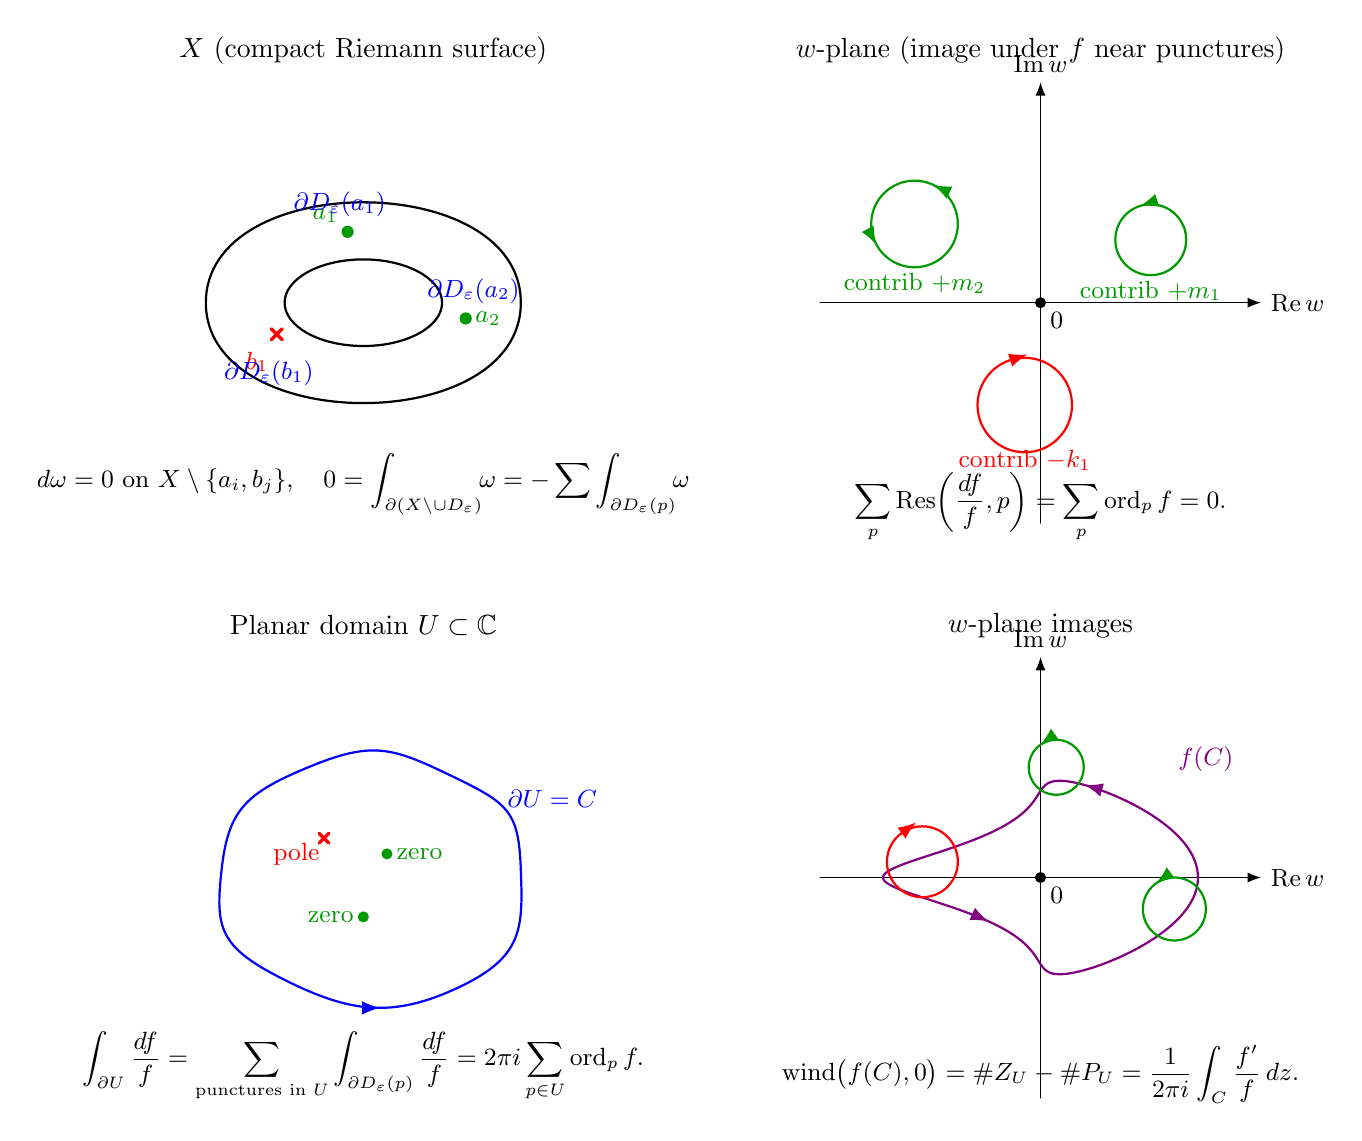
\begin{tikzpicture}[>=Latex, line cap=round, line join=round, font=\small]
	
	% ===============================
	% ========== TOP ROW ============
	% Compact Riemann surface X (torus) and image loops in w-plane
	% ===============================
	
	% ---- Left: compact surface X with punctures ----
	\begin{scope}[shift={(0,0)}]
		\node[font=\normalsize] at (0,3.2) {$X$ (compact Riemann surface)};
		
		% crude torus silhouette: outer and inner loops
		\draw[thick] (-2,0) .. controls (-2,1.7) and (2,1.7) .. (2,0)
		.. controls (2,-1.7) and (-2,-1.7) .. (-2,0);
		\draw[thick,fill=white] (0,0) ellipse (1.0 and 0.55);
		
		% mark zeros (green) and poles (red) on X
		\fill[green!60!black] (-0.2,0.9) circle(2.2pt) node[above left] {$a_1$};
		\fill[green!60!black] (1.3,-0.2) circle(2.2pt) node[right] {$a_2$};
		\draw[red,very thick] (-1.1,-0.4) ++(-0.07,-0.07) -- ++(0.14,0.14);
		\draw[red,very thick] (-1.1,-0.4) ++(-0.07,0.07) -- ++(0.14,-0.14);
		\node[red] at (-1.35,-0.75) {$b_1$};
		
		% excised small disks around a_i, b_j (inner boundaries clockwise)
%		\foreach \P in {(-0.2,0.9),(1.3,-0.2),(-1.1,-0.4)}{
%			\draw[blue,thick,postaction={decorate},
%			decoration={markings, mark=at position 0.15 with {\arrow{<}}}]
%			(\P) circle (0.28);
%		}
		\node[blue] at (-0.3,1.25) {$\partial D_\varepsilon(a_1)$};
		\node[blue] at (1.4,0.15) {$\partial D_\varepsilon(a_2)$};
		\node[blue] at (-1.2,-0.9) {$\partial D_\varepsilon(b_1)$};
		
		% Stokes annotation
		\node[align=center] at (0,-2.3)
		{$\displaystyle d\omega=0\ \text{on}\ X\setminus\{a_i,b_j\},\quad
			0=\int_{\partial( X\setminus\cup D_\varepsilon)}\!\!\omega
			=-\sum\int_{\partial D_\varepsilon(p)}\!\!\omega$};
	\end{scope}
	
	% ---- Right: w-plane image loops (around 0) ----
	\begin{scope}[shift={(8.6,0)}]
		\node[font=\normalsize] at (0,3.2) {$w$-plane (image under $f$ near punctures)};
		\draw[->] (-2.8,0)--(2.8,0) node[right] {$\Re w$};
		\draw[->] (0,-2.8)--(0,2.8) node[above] {$\Im w$};
		\fill (0,0) circle(2pt) node[below right] {$0$};
		
		% loops for two zeros: CCW with multiplicities m1=1, m2=2 (as example)
		% (we just show CCW loops labeled +m)
		\draw[green!60!black,thick,postaction={decorate},
		decoration={markings, mark=at position 0.3 with {\arrow{>}}}]
		(1.4,0.8) circle (0.45);
		\node[green!60!black] at (1.4,0.15) {contrib $+m_1$};
		
		\draw[green!60!black,thick,postaction={decorate},
		decoration={markings, mark=at position 0.18 with {\arrow{>}},
			mark=at position 0.58 with {\arrow{>}}}]
		(-1.6,1.0) circle (0.55);
		\node[green!60!black] at (-1.6,0.25) {contrib $+m_2$};
		
		% loop for one pole: CW with multiplicity k=2 (example)
		\draw[red,thick,postaction={decorate},
		decoration={markings, mark=at position 0.3 with {\arrow{<}}}]
		(-0.2,-1.3) circle (0.6);
		\node[red] at (-0.2,-2.0) {contrib $-k_1$};
		
		% caption: residues sum to zero
		\node[align=center] at (0,-2.6)
		{$\displaystyle \sum_{p}\operatorname{Res}\!\left(\frac{df}{f},p\right)
			= \sum_{p}\operatorname{ord}_p f = 0.$};
	\end{scope}
	
	% ===============================
	% ======== BOTTOM ROW ===========
	% Planar domain version: domain in z-plane and image in w-plane
	% ===============================
	
	% ---- Left: planar domain with outer boundary C and inner circles ----
	\begin{scope}[shift={(0,-7.3)}]
		\node[font=\normalsize] at (0,3.2) {Planar domain $U\subset\mathbb{C}$};
		% outer boundary C
		\draw[blue,thick,postaction={decorate},
		decoration={markings, mark=at position 0.6 with {\arrow{>}}}]
		plot[smooth cycle, tension=1]
		coordinates{(2.0,0.1) (1.1,1.3) (-0.7,1.4) (-1.8,0.1) (-1.0,-1.3) (1.2,-1.4)};
		\node[blue] at (2.4,1.0) {$\partial U=C$};
		
		% inner small circles (punctures) oriented clockwise
%		\foreach \Q in {(0.3,0.3),(-0.5,0.5),(0.0,-0.5)}{
%			\draw[blue,thick,postaction={decorate},
%			decoration={markings, mark=at position 0.2 with {\arrow{<}}}]
%			(\Q) circle (0.25);
%		}
		
		% mark zeros/poles inside
		\fill[green!60!black] (0.3,0.3) circle(2pt) node[right] {$\text{zero}$};
		\draw[red,very thick] (-0.5,0.5) ++(-0.06,-0.06) -- ++(0.12,0.12);
		\draw[red,very thick] (-0.5,0.5) ++(-0.06,0.06) -- ++(0.12,-0.12);
		\node[red] at (-0.85,0.3) {$\text{pole}$};
		\fill[green!60!black] (0.0,-0.5) circle(2pt) node[left] {$\text{zero}$};
		
		% annotation
		\node[align=center] at (0,-2.4)
		{$\displaystyle \int_{\partial U}\frac{df}{f}
			= \sum_{\text{punctures in }U}\int_{\partial D_\varepsilon(p)}\frac{df}{f}
			= 2\pi i \sum_{p\in U}\operatorname{ord}_p f.$};
	\end{scope}
	
	% ---- Right: image w-plane of the boundaries ----
	\begin{scope}[shift={(8.6,-7.3)}]
		\node[font=\normalsize] at (0,3.2) {$w$-plane images};
		\draw[->] (-2.8,0)--(2.8,0) node[right] {$\Re w$};
		\draw[->] (0,-2.8)--(0,2.8) node[above] {$\Im w$};
		\fill (0,0) circle(2pt) node[below right] {$0$};
		
		% image of outer boundary C under f: some loop (violet)
		\draw[violet,thick,
		postaction={decorate},
		decoration={markings, mark=at position 0.2 with {\arrow{>}},
			mark=at position 0.65 with {\arrow{>}}}]
		plot[domain=0:6.283, samples=220]
		({1.6*cos(\x r)+0.4*cos(3*\x r)},
		{1.1*sin(\x r)+0.3*sin(2*\x r)});
		\node[violet] at (2.1,1.5) {$f(C)$};
		
		% images of small circles: loops around 0 with signs
		\draw[green!60!black,thick,postaction={decorate},
		decoration={markings, mark=at position 0.35 with {\arrow{>}}}]
		(1.7,-0.4) circle (0.4);  % zero -> CCW
		\draw[red,thick,postaction={decorate},
		decoration={markings, mark=at position 0.35 with {\arrow{<}}}]
		(-1.5,0.2) circle (0.45); % pole -> CW
		\draw[green!60!black,thick,postaction={decorate},
		decoration={markings, mark=at position 0.35 with {\arrow{>}}}]
		(0.2,1.4) circle (0.35);  % zero -> CCW
		
		\node[align=center] at (0,-2.5)
		{$\displaystyle \mathrm{wind}\big(f(C),0\big)
			= \#Z_U-\#P_U
			= \frac{1}{2\pi i}\int_{C}\frac{f'}{f}\,dz.$};
	\end{scope}
	
\end{tikzpicture}
\end{document}
